%======================================================================
\chapter{Variational derivatives}\label{app:derivatives}
%======================================================================
% Source: slides L01 "Variational calculus" (functional, Gateaux,
% Frechet, functional derivative, problem settings, exercises).

\framepart{Outline}
This appendix collects the technical definitions behind the first variation
used throughout Chapter~\ref{ch:var}: the G\^ateaux and Fr\'echet derivatives
of a functional, the functional derivative, and the Euler--Lagrange equations
of integral functionals. Standard references are~\cite{GelfandFomin,DacorognaIntro}.

%======================================================================
\section{Energy functionals}
Let
\begin{itemize}
  \item $V$ be a functional space (a normed vector space, typically a Sobolev
  space) and $V^\ast$ its dual, the space of continuous linear forms on $V$;
  \item $\scal{\cdot}{\cdot}:V^\ast\times V\to\R$ the duality pairing;
  \item $\mathcal W:V\to\R$ a functional, typically an energy;
  \item $u_0\in V$ a point: a displacement field, a temperature field, \dots
\end{itemize}
The objective is to compute a derivative of $\mathcal W$ at $u_0$, i.e.\ a
first-order linear approximation, in the spirit of a Taylor expansion
\[
  \mathcal W(u_0+\delta u)=\mathcal W(u_0)+\delta\mathcal W(u_0)[\delta u]+\cdots
\]

%======================================================================
\section{G\^ateaux and Fr\'echet derivatives}
\begin{gbox}{Derivatives of a functional}
\index{Gateaux derivative@G\^ateaux derivative}\index{Frechet derivative@Fr\'echet derivative}\index{functional derivative}\index{first variation}%
\begin{description}[style=nextline,leftmargin=1em,font=\sffamily\bfseries]
\item[G\^ateaux (weak, directional) derivative]
\begin{equation}\label{eq:gateaux}
  \delta\mathcal W(u_0)[v]=\lim_{\alpha\to0}\frac{\mathcal W(u_0+\alpha v)-\mathcal W(u_0)}{\alpha}
  =\frac{\dd}{\dd\alpha}\mathcal W(u_0+\alpha v)\Big|_{\alpha=0} .
\end{equation}
$\mathcal W$ is \emph{G\^ateaux differentiable} at $u_0$ if this limit exists for
every direction $v$ and $v\mapsto\delta\mathcal W(u_0)[v]$ is linear and
continuous.
\item[Fr\'echet (strong) derivative]
a continuous linear map $D\mathcal W(u_0)\in V^\ast$ such that
\begin{equation}\label{eq:frechet}
  \lim_{\norm{v}\to0}\frac{\mathcal W(u_0+v)-\mathcal W(u_0)-D\mathcal W(u_0)\,v}{\norm{v}}=0 .
\end{equation}
\item[Functional derivative]
$\dfrac{\delta\mathcal W}{\delta u}(u_0)$, the object representing the first
variation through the pairing (in practice, the $L^2$ inner product):
\begin{equation}\label{eq:functional-derivative}
  \delta\mathcal W(u_0)[\eta]=\Bigl\langle\frac{\delta\mathcal W}{\delta u}(u_0),\eta\Bigr\rangle
  \qquad\forall\eta\in V .
\end{equation}
\end{description}
\end{gbox}

\paragraph{Relations.} A Fr\'echet derivative is a G\^ateaux derivative: take
$v=\alpha w$ in~\eqref{eq:frechet}. The converse is false. The limit in
\eqref{eq:gateaux} is taken along straight lines through $u_0$ only, while
\eqref{eq:frechet} requires a uniform approximation in all directions at
once. If the G\^ateaux derivative exists in a neighbourhood of $u_0$ and is
continuous in $u_0$ (as a map into $V^\ast$), then $\mathcal W$ is Fr\'echet
differentiable. For the quadratic energies of this book both derivatives
exist and coincide; the distinction matters for non-smooth or non-convex
energies.

\paragraph{Two examples in $\R^2$} (Figure~\ref{fig:gateaux}).
\index{Gateaux derivative@G\^ateaux derivative!vs Fr\'echet}%
\begin{itemize}
\item $g_1(x,y)=\dfrac{x^2y}{x^2+y^2}$, $g_1(0,0)=0$. Along a direction
$\vv=(v_1,v_2)$, $g_1(\alpha\vv)/\alpha=v_1^2v_2/|\vv|^2$: all directional
derivatives exist at the origin, but $\vv\mapsto v_1^2v_2/|\vv|^2$ is not
linear. $g_1$ is not G\^ateaux differentiable in the sense above.
\item $g_2(x,y)=\dfrac{x^3y}{x^4+y^2}$, $g_2(0,0)=0$. Along a direction,
$g_2(\alpha\vv)/\alpha=\alpha\,v_1^3v_2/(\alpha^2v_1^4+v_2^2)\to0$: the G\^ateaux
derivative exists and is zero, hence linear. But along the parabola
$y=x^2$, $g_2=x/2$, so $g_2(x,x^2)/|(x,x^2)|\to\tfrac12\neq0$: $g_2$ is not
Fr\'echet differentiable at the origin, although it is continuous there
($|g_2|\le|x|/2$).
\end{itemize}
\begin{figure}[h]
\centering
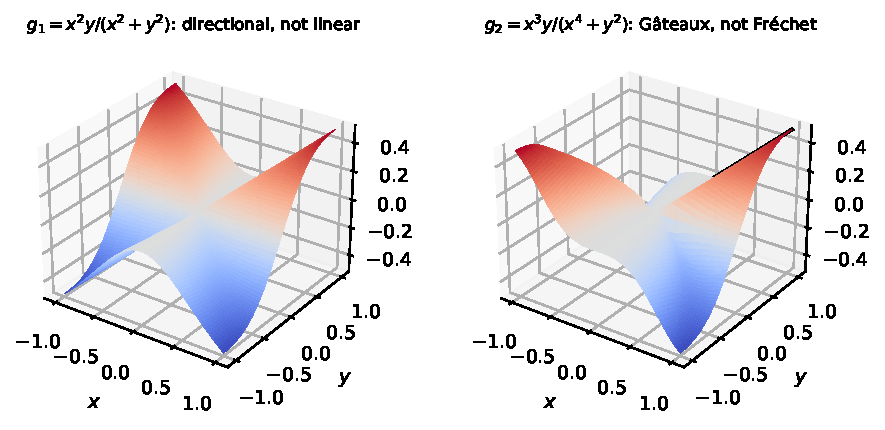
\includegraphics[width=\textwidth]{figures/appA/gateaux_frechet.pdf}
\caption{Left: $g_1$ has directional derivatives at the origin which are not
linear in the direction. Right: $g_2$ is G\^ateaux differentiable at the
origin (zero derivative along every straight line), but not Fr\'echet
differentiable: along the parabola $y=x^2$ (black curve) it grows like $x/2$.}
\label{fig:gateaux}
\end{figure}

%======================================================================
\section{Three equivalent problem settings}
\begin{gbox}{Problem settings}
\index{weak form}\index{strong form}\index{energy!minimization}%
\begin{description}[style=nextline,leftmargin=1em,font=\sffamily\bfseries]
\item[Energy minimization] Find $u_0$ minimizing $\mathcal W(u)$ over $V$.
\item[Weak formulation (virtual work)]
\[
  \delta\mathcal W(u_0)[v]=0\quad\forall v\in V,
  \qquad\text{or}\qquad
  \Bigl\langle\frac{\delta\mathcal W}{\delta u}(u_0),v\Bigr\rangle=0\quad\forall v\in V .
\]
\item[Strong formulation (Euler--Lagrange equations)]
\[
  \frac{\delta\mathcal W}{\delta u}(u_0)=0 .
\]
\end{description}
\end{gbox}
A minimizer satisfies the weak form (the first variation vanishes at a
minimum); for a convex $\mathcal W$ the converse holds. The difference between
the two weak forms lies in the derivatives of $v$: the first contains
derivatives of $v$, the second none, after integration by parts. Passing from
the weak to the strong form requires this integration by parts and enough
regularity of $u_0$.

%======================================================================
\section{Integral functionals and the Euler--Lagrange equations}
Let $\mathcal W(u)=\int_\Omega\mathcal F(\vx,u,\nabla u)\dd x$, with
$\mathcal F$ smooth. Differentiating under the integral,
\[
  \delta\mathcal W(u)[v]=\int_\Omega\Bigl(\frac{\partial\mathcal F}{\partial u}\,v
  +\frac{\partial\mathcal F}{\partial(\nabla u)}\cdot\nabla v\Bigr)\dd x .
\]
Integrating the second term by parts (Theorem~\ref{thm:ibp}):
\[
  \delta\mathcal W(u)[v]=\int_\Omega\Bigl(\frac{\partial\mathcal F}{\partial u}
  -\dive\frac{\partial\mathcal F}{\partial(\nabla u)}\Bigr)v\dd x
  +\int_{\partial\Omega}\frac{\partial\mathcal F}{\partial(\nabla u)}\cdot\vn\,v\dd s .
\]
\begin{gbox}{Euler--Lagrange equations}
\index{Euler--Lagrange equation}\index{boundary condition!natural}%
\begin{equation}\label{eq:EL}
  \frac{\delta\mathcal W}{\delta u}=\frac{\partial\mathcal F}{\partial u}
  -\dive\frac{\partial\mathcal F}{\partial(\nabla u)}=0\ \ \text{in }\Omega,
  \qquad
  \frac{\partial\mathcal F}{\partial(\nabla u)}\cdot\vn=0\ \ \text{where $u$ is not prescribed.}
\end{equation}
The boundary condition is \emph{natural}; where $u$ is prescribed, $v=0$ and
there is no condition.
\end{gbox}

\paragraph{General first-order operators.} More generally, let
\index{adjoint operator!formal}\index{beam!Euler--Bernoulli}%
$\mathcal W(u)=\int_\Omega\mathcal F(Du)\dd x$ with $D$ a linear differential
operator (components $D_i$). Then
\[
  \delta\mathcal W(u)[v]=\int_\Omega\frac{\partial\mathcal F}{\partial(D_iu)}\,D_iv\dd x=0
  \quad\forall v
  \qquad\Longleftrightarrow\qquad
  D_i^\ast\frac{\partial\mathcal F}{\partial(D_iu)}=0,
\]
where $D^\ast$ is the formal adjoint of $D$, defined by
$\int_\Omega(Du)\cdot w=\int_\Omega u\,D^\ast w$ for fields vanishing on the
boundary. The pairs used in this book are:
\begin{center}
\renewcommand{\arraystretch}{1.25}
\begin{tabular}{llll}
\toprule
\sffamily operator $D$ & \sffamily adjoint $D^\ast$ & \sffamily energy density & \sffamily Euler--Lagrange\\
\midrule
$\nabla$ (scalar) & $-\dive$ & $\tfrac12\nabla u\cdot\tk\nabla u-fu$ & $-\dive(\tk\nabla u)=f$\\
$\eps[\cdot]=\sym\nabla$ & $-\dive$ (on symmetric tensors) & $\tfrac12\eps:\bbC:\eps-\vf\cdot\vu$ & $-\dive(\bbC:\eps[\vu])=\vf$\\
$\dd/\dd x$ & $-\dd/\dd x$ & $\tfrac12EA(u')^2-fu$ & $-(EAu')'=f$\\
$\dd^2/\dd x^2$ & $\dd^2/\dd x^2$ & $\tfrac12EI(w'')^2-qw$ & $(EIw'')''=q$\\
$\mat{B}$ (matrix) & $\mat{B}\T$ & $\tfrac12\mat{B}\vu\cdot\mat{C}\mat{B}\vu-\vf\cdot\vu$ & $\mat{B}\T\mat{C}\mat{B}\vu=\vf$\\
\bottomrule
\end{tabular}
\end{center}
The last line is the spring chain of Section~\ref{sec:var-discrete}: the
adjoint of a differential operator is the continuum counterpart of the
transpose of a matrix.

%======================================================================
\section{Second variation and convexity}
\index{second variation}\index{convexity}%
The second G\^ateaux derivative,
$\delta^2\mathcal W(u)[v,w]=\frac{\partial^2}{\partial\alpha\,\partial\beta}\mathcal W(u+\alpha v+\beta w)\big|_{0}$,
is symmetric in $(v,w)$ when it exists and is continuous (Schwarz). This is
why a non-symmetric bilinear form cannot be the second variation of an energy
(Exercise~\ref{exo:no-energy}). If $\delta^2\mathcal W(u)[v,v]\ge0$ for all
$u,v$, $\mathcal W$ is convex and every critical point is a minimizer; if
$\delta^2\mathcal W(u)[v,v]\ge\alpha\norm{v}^2$, the minimizer is unique. A
critical point at which the second variation takes negative values is
unstable (the double well of Section~\ref{sec:var-lm}).

%======================================================================
\framepart{Summary}
\begin{gbox*}
\begin{itemize}
  \item The \textbf{G\^ateaux derivative} is the derivative along straight
  lines, $\frac{\dd}{\dd\alpha}\mathcal W(u_0+\alpha v)|_{\alpha=0}$; the
  \textbf{Fr\'echet derivative} is a uniform linear approximation. Fr\'echet
  implies G\^ateaux, not conversely.
  \item An energy problem has three settings: \textbf{minimization},
  \textbf{weak form} ($\delta\mathcal W(u)[v]=0$ for all $v$) and
  \textbf{strong form} ($\delta\mathcal W/\delta u=0$, the Euler--Lagrange
  equations, with natural boundary conditions).
  \item For $\mathcal W=\int\mathcal F(Du)$ the Euler--Lagrange operator is
  $D^\ast\,\partial\mathcal F/\partial(Du)$: the formal adjoint of a
  differential operator plays the role of the transpose of a matrix.
  \item The \textbf{second variation} is symmetric; its sign decides
  convexity, uniqueness and stability.
\end{itemize}
\end{gbox*}

\framepart{Exercises}

\exercise{A membrane, or steady heat conduction}\label{exo:A-membrane}
Find the three problem settings for
\[
  \mathcal W(u)=\int_\Omega\Bigl[\frac c2\Bigl(\frac{\partial u}{\partial x}\Bigr)^2
  +\frac c2\Bigl(\frac{\partial u}{\partial y}\Bigr)^2-fu\Bigr]\dd x\dd y,
  \qquad\Omega\subset\R^2 .
\]
Give a physical interpretation of the fields.
\begin{solution}
Minimization of $\mathcal W$ over $u$ (with $u$ given on part of the boundary).
Weak form: $\int_\Omega(c\nabla u\cdot\nabla v-fv)=0$ for all admissible $v$.
Strong form: $-c\Delta u=f$ in $\Omega$, $c\,\partial_nu=0$ where $u$ is free.
Interpretations: transverse deflection $u$ of a membrane of tension $c$ under
a pressure $f$; temperature $u$ in a plate of conductivity $c$ with heat
source $f$; Prandtl stress function of a twisted bar ($f=2\mu\theta$).
\end{solution}

\exercise{From the strong form back to the energy}\label{exo:A-pendulum}
The strong formulation of a problem is $-u''+\sin u=0$,
$u:\R\to\R$. Find its weak formulation and its energy functional.
\begin{solution}
Weak form: $\int(u'v'+\sin u\,v)\dd x=0$ for all $v$ with compact support.
Since $\sin u=\frac{\dd}{\dd u}(-\cos u)$, the energy is
$\mathcal W(u)=\int\bigl(\tfrac12(u')^2-\cos u\bigr)\dd x$ (up to a constant).
With $x$ read as time it is the action of a pendulum,
$\int(\text{kinetic}-\text{potential})$ with potential $\cos u$, i.e.\ an inverted
pendulum; it is also the static sine-Gordon equation for a chain of torsion
springs. The energy is not convex: $\delta^2\mathcal W(u)[v,v]=\int((v')^2+\cos u\,v^2)$
can be negative.
\end{solution}

\exercise{Minimal surfaces}\label{exo:A-minimal}
Find the three problem settings for
\[
  \mathcal W(u)=\int_\Omega\Bigl[1+\Bigl(\frac{\partial u}{\partial x}\Bigr)^2
  +\Bigl(\frac{\partial u}{\partial y}\Bigr)^2\Bigr]^{1/2}\dd x\dd y,
  \qquad u=u_0\ \text{on }\partial\Omega .
\]
Give a physical interpretation. Hint:
$(1+a+b)^{1/2}=(1+a)^{1/2}+\frac{b}{2(1+a)^{1/2}}+O(b^2)$.
\begin{solution}
$\mathcal W$ is the area of the graph of $u$. With
$a=|\nabla u|^2$ and $b=2\alpha\nabla u\cdot\nabla v+\alpha^2|\nabla v|^2$, the hint
gives
$\delta\mathcal W(u)[v]=\int_\Omega\frac{\nabla u\cdot\nabla v}{\sqrt{1+|\nabla u|^2}}=0$
for all $v$ vanishing on $\partial\Omega$ (weak form), and
$\dive\bigl(\nabla u/\sqrt{1+|\nabla u|^2}\bigr)=0$ (strong form, the minimal
surface equation). The left-hand side is twice the mean curvature of the
graph: a soap film spanning the wire $u_0$ has zero mean curvature
(Section~\ref{sec:var-phys}). For small slopes, $\mathcal W\approx|\Omega|+\tfrac12\int|\nabla u|^2$
and the equation linearizes to $\Delta u=0$.
\end{solution}

\exercise{Derivative of the elastic energy}\label{exo:A-elastic}
Compute the G\^ateaux derivative of
$\mathcal U(\vu)=\int_\Omega\tfrac12\eps[\vu]:\bbC:\eps[\vu]\dd x$ and show that
it is a Fr\'echet derivative on $H^1(\Omega)^3$.
\begin{solution}
$\mathcal U(\vu+\alpha\vv)=\mathcal U(\vu)+\alpha\int\eps[\vu]:\bbC:\eps[\vv]+\alpha^2\mathcal U(\vv)$
by the major symmetry of $\bbC$, so
$\delta\mathcal U(\vu)[\vv]=\int_\Omega\eps[\vu]:\bbC:\eps[\vv]$, linear and bounded
in $\vv$. The remainder is $\mathcal U(\vv)\le\tfrac12|\bbC|\,\norm{\vv}_{H^1}^2=o(\norm{\vv})$:
the derivative is Fr\'echet.
\end{solution}

%======================================================================
\begin{chapterbib}{9}
\bibitem{DacorognaIntro} B.~Dacorogna, \emph{Introduction to the Calculus of Variations}, 3rd ed., Imperial College Press, 2015.
\bibitem{GelfandFomin} I.~M.~Gelfand, S.~V.~Fomin, \emph{Calculus of Variations}, Prentice-Hall, 1963 (Dover reprint, 2000).
\end{chapterbib}
